\week{Data}

Get out a piece of paper and draw a duck. It can be any kind of duck you want, in whatever pose.

Once you're done, have your friend take out a new sheet of paper. Without showing them your drawing,
describe exactly what you drew and have them attempt to replicate it.

How did they do? If you're like most people, you probably gave directions that were vague enough to
be interpreted in many ways. Your friend's drawing probably doesn't look a whole lot like yours.

\begin{marginfigure}
  \centering
  \includegraphics[width=0.8\marginparwidth]{../week2/figures/duck.jpg}
  \caption{Can you describe exactly how to draw this duck? Your computer can!}
\end{marginfigure}

In casual conversation, we often mix up our own ideas of how things ought to be with the way things
are. None of the instructions you gave about how to draw your duck were wrong, and the drawing your
friend made from them is also not wrong. They just highlight different parts of how \emph{you}
interpreted your own drawing and how \emph{they} interpreted your description of it.\didyouknow{Many of the products we use today are
  made by computers that manipulate real life materials, like wood,
  metals, and plastic. Precise instructions are provided to these
  machines using a special computer unit called a \term{Computer
    Numerical Control} (or \term{CNC} module) that produce highly-detailed pieces like the one shown here.

  \includegraphics[width=0.8\marginparwidth]{../week2/figures/cnc-machine.jpg}
  \attribution{Cameronm125, CC BY-SA 4.0 <https://creativecommons.org/licenses/by-sa/4.0>, via Wikimedia Commons}
  }

When it comes to computers, we have to describe things exactly, because computers simply follow
rules. If the instructions you gave your friend were not clear, your friend probably figured out a
meaning that made sense to them. Computers don't do that. They simply do exactly as they are told.

\section{Week 1 Review}

Last week, we discussed how certain machines obey rules. Once the rules are set up, the machine
always obeys those rules. We constructed machines last week that counted marbles. We counted out the
right number of marbles by manipulating switches on a board. The orientation of these switches
determined how many marbles would fall.

Computers also use switches to store numbers. Each switch in a computer can be on or off, or a ``1''
or ``0''. Any combination of 1s and 0s can be used to write a number in binary form.

All of these principles are based on fixed rules.

We saw that Python also follows rules. Python can manipulate numbers and words. Although numbers are
stored internally in a binary form, Python interprets them for us, so that we can talk to it using
the numbers we're familiar with. Python has rules for converting numbers back into binary form and
also for manipulating words.

We also saw that Python has rules regarding what kind of things it can
talk about. When we mistyped something in Python, we get something
called an error. See \prettyref{tab:python-errors} for a list of
errors we may see this week.

\begin{table}
  \fixfigure

\begin{tabularx}{\linewidth}{lp{0.5\linewidth}}
\toprule
\code{NameError} & A name of a rule was mistyped (i.e., you typed \code{length} instead of \code{len}). \\
\code{TypeError} & You used a number where a word was expected or vice versa (i.e., \code{'hello'/2}). \\
\code{ZeroDivisionError} & You tried to divide a number by zero. Uh-oh! \\
\code{SyntaxError} & Python couldn't make sense of what you typed because it didn't follow Python's rules (i.e., you typed \code{2 + 5 *} and python doesn't know what to multiply 5 by). \\
\code{OverflowError} & Some kinds of calculations on numbers can result in very large numbers that don't fit into the computer. \\\bottomrule
\end{tabularx}

\caption{As we continue in our learning, we will most likely encounter more errors. Errors are a
  \emph{normal} part of programming. They do not mean anything is broken! It just means there's been
  a misunderstanding between what you thought was going to happen and what actually happened when
  the computer followed through exactly with the rules you set out for it. Instead of being
  discouraged, think of every error as an opportunity learn \emph{more}!}
\label{tab:python-errors}
\end{table}

\section{Numbers All the Way Down}

Last week, we discussed how computers store numbers using switches that are either on or
off. \hint{See \prettyref{sec:binary-numbers} for a review.}

Everything on a computer is stored as numbers. Even the words we saw last class are stored using
numbers. Every letter in a word (or a \term{string} as Python calls it) is assigned a number. We
call these numbers the \term{encoding} of the string.\hint{Python will sometimes abbreviate \term{string} as \code{str}.}

Most modern computers today use the \term{Unicode} standard for encoding strings. Unicode is a
\emph{huge} dictionary mapping every character possibly known to humans to a number assigned by an
international committee.\didyouknow{As of the latest Unicode standard, there are over 297,334
  characters! That's a lot of letters!} Before Unicode standardized the mapping of characters,
computer systems would often use their own custom standard or a standard particular to individual
countries and languages. Reading files created using one standard on a computer designed to work
with another standard could result in garbage data. Another common way to write strings as numbers
is called \term{ASCII}, which stands for the \emph{American Standard Code for Information
Interchange}. ASCII covers most characters used in English and other languages that use the Latin
alphabet. It's also compatible with Unicode -- Unicode maps every Latin letter to the same ASCII
character.

It may seem crazy that each letter has a number that goes along with it, but I can prove it to you. Try this in Python:

\hint{If you want to see a new kind of error called a \code{ValueError}, try\\
\code{ord('hello')}!}
\begin{replbox}
>>> ord('5')<ENTER>
53
>>> ord('Z')<ENTER>
90
>>> ord('>')<ENTER>
62
>>> ord('\'')<ENTER>(*@ \tikzmarknode{python escapes node}{} @*)
39
>>> ord('h')<ENTER>
104
\end{replbox}
\makemargmark{python escapes node}{\notestyle\hintnote Python words are delimited by single quotation marks (\code{'}). But what if you want to talk about the word consisting of just the single quote character itself or a word containing a single quote character (like an Irish name with \enquote{O'})? In order to tell Python that you want a \code{'} treated as just the letter and not part of the Python rules, you use the \code{\textbackslash} character in front of it. This word \code{'\textbackslash''} is just the word consisting of a single single-quote letter.}
%}


You can also go from a number \emph{to} a word.

\hint{Try all kinds of numbers here, and see what you get!}
\begin{replbox}
>>> chr(76)<ENTER>
'L'
>>> chr(53)<ENTER>
'5'
>>> chr(54)<ENTER>
'6'
>>> chr(233)<ENTER>
'é'
>>> chr(1103)<ENTER>
'я'
>>> chr(26159)<ENTER>
'是'
>>> chr(22398)<ENTER>
'学'(*@\tikzmarknode{chinese xie}{}@*)
>>> chr(128512)<ENTER>
'(*@{\EmojiFont 😀}@*)'
\end{replbox}
\makemargmark{chinese xie}{\hintnote \enquote{学}(\emph{xi\`e}) means to learn in Mandarin. That's what we're doing right now, and you just learned something new!}

Lest we forget that it's still all just ones and zeros, you can use the \code{bin} rule that we
learned about last week to see the binary representation of these numbers.

\begin{replbox}
>>> bin(ord('5'))<ENTER>
'0b100111'(*@\tikzmarknode{single quotes around binary numbers}{}@*)
>>> bin(ord('Z'))<ENTER>
'0b1011010'
>>> bin(ord('\''))<ENTER>
'0b100111'
\end{replbox}
\makemargmark{single quotes around binary numbers}{\notestyle\huhnote{I thought the single quotes meant words. Why do we keep seeing them when we ask for binary numbers?}\\
Because Python is friendly, it always shows numbers as decimal, even though they are stored as binary on the computer. The \code{bin} rule actually creates a word, or string, that represents the binary representation. This lets you see it here.}

See it's just numbers all the way down!

\begin{BigIdeaBox}
  All information inside a modern computer is stored as numbers, even words!
\end{BigIdeaBox}

\section{Drawing a Very Precise Duck}

\begin{marginfigure}
  \centering
  \begin{tikzpicture}
    \draw (0,0) pic[duck/water=blue] {duck};
  \end{tikzpicture}
  \caption{This is a very precise duck!}
  \label{fig:precise-duck}
\end{marginfigure}

Think back to the duck exercise we did at the beginning of class. We
found it was hard to describe a duck perfectly to our friend. But that's because we didn't know
\emph{how} to describe a duck properly. We weren't \emph{precise} enough.

\begin{BigIdeaBox}
English is a great language for everyday communication, but it is not great at being exact about
visual information. To talk about drawings, we need a language that allows us to be precise about something.
\end{BigIdeaBox}

Whenever we want to describe something in detail, we have to understand how to be precise about
it. Switches are precise -- they are either on or off. Numbers are precise too, because they can be
represented by a bunch of switches. We need a way of turning an image into numbers.

%\begin{marginfigure}
%  \centering
%  \includegraphics[width=0.8\marginparwidth]{../week2/figures/plato.jpg}
%  \caption{The Greek philosopher \textbf{Plato} believed that things
%    existed before being described.}
%\end{marginfigure}

% \begin{TrackBox}{Gaming}
%   Some computer scientists try to match the descriptions and names on
%   the computer match those they observe in the real world. When we do
%   this, we can use the computer to predict what would happen. This is
%   called a \term{simulation}.
% \end{TrackBox}


\begin{TrackBox}{Graphics}
  \boxtitle{How Computers Draw}

Computers draw using -- you guessed it -- numbers! You've probably seen the \term{number line} in
your math courses. All numbers can be placed on a simple line, and we can name any point on the line
by writing down a number to name it.

%\makemargmark{number line
%  comment}{\notestyle \huhnote{This coordinate system looks different than my math courses! What's
%    going on?}{If you've done geometry you've probably seen the cartesian plane drawn with the $y$
%    coordinate increasing as you go up. On many computers, the $y$ coordinate increases as you go
%    \emph{down}. Computers often use this different coordinate system so that the coordinates match
%    how things are physically drawn. It doesn't matter which system you choose, as long as everyone
%    does it the same way. In both systems, each grid is named by a unique number.}}

But to make graphics, we need to be able to talk about \tikzmarknode{points on a screen}{points} on
a rectangular screen, not a line. How do we name a point on a rectangle? The first person to think
about this systematically was a scientist, mathematician, and philosopher named \textbf{Ren\'e
  Descartes} who invented \emph{Cartesian plane}. Here's how it works. Instead of a line, we draw a
grid. We number all the columns and all the rows (see \prettyref{fig:cartesian-grid}). Now, any
square on the grid can be named by giving two numbers. These two numbers together are called the
\term{coordinate}. We usually write the \emph{column} number first, and the \emph{row} number
last. This system is called the \emph{cartesian coordinate} system.

\makemargmark{points on a screen}{
  \par\medskip
  % Requires:
% \usepackage{tikz}
% \usetikzlibrary{calc}

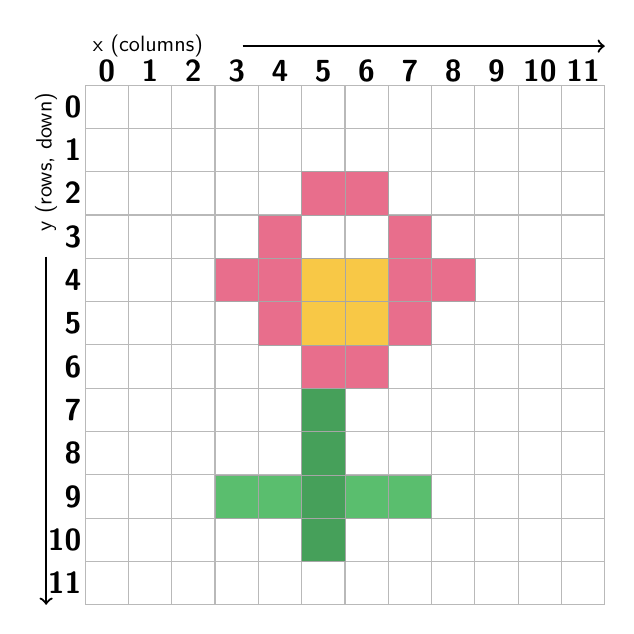
\begin{tikzpicture}[
  font=\sffamily,
  x=0.55cm, y=0.55cm, % pixel size
  line join=round
]
  % ---- grid size ----
  \def\W{12} % number of columns
  \def\H{12} % number of rows

  % ---- background ----
  \fill[white] (0,0) rectangle (\W,\H);

  % ---- draw grid ----
  \draw[step=1, gray!55] (0,0) grid (\W,\H);

  % ---- axis labels: x left->right, y top->bottom ----
  % Column indices along top: 0..W-1
  \foreach \x in {0,...,11} {
    \node[anchor=south, scale=1.1, font=\bfseries\sffamily, inner sep=1pt] at (\x+0.5, \H) {\x};
  }
  % Row indices along left, with y increasing downward:
  % Put 0 at the top row (near y=H-0.5), then 1 below it, ...
  \foreach \y in {0,...,11} {
    \node[anchor=east, scale=1.1, font=\bfseries\sffamily, inner sep=1pt] at (0, \H-\y-0.5) {\y};
  }

  % Optional axis titles
  \node[anchor=west, scale=0.8] at (0, \H+0.9) {x (columns)};
  \draw[->,line width=0.8pt] (2cm, \H+0.9) -s (\W,\H+0.9);
  \node[anchor=east, scale=0.8, rotate=90] at (-0.9, \H) {y (rows, down)}; % name this node Y
  \draw[->,line width=0.8pt] (-0.9, \H+4cm) -- (-0.9, 0); % start this at the south of Y offset by 0.5 downwards and continue it down

  % ---- helper: draw a pixel at (x,y) where y=0 is top row ----
  % We'll just place rectangles manually using the mapping:
  % pixel (x,y) -> rectangle from (x, H-y-1) to (x+1, H-y)

  % Colors
  \definecolor{petal}{RGB}{232,110,140}
  \definecolor{center}{RGB}{248,200,70}
  \definecolor{stem}{RGB}{70,160,90}
  \definecolor{leaf}{RGB}{90,190,110}

  % ---- flower pixels ----
  % petals (a chunky 5x5-ish flower head)


  % Petals (explicit, simpler)
  \foreach \x/\y in {
    5/2, 6/2,
    4/3, 7/3,
    3/4, 8/4,
    4/5, 7/5,
    5/6, 6/6,
    5/4, 6/4, 4/4, 7/4 % make it fuller
  }{
    \fill[petal] (\x, \H-\y-1) rectangle (\x+1, \H-\y);
  }

  % center
  \foreach \x/\y in {5/4,6/4,5/5,6/5} {
    \fill[center] (\x, \H-\y-1) rectangle (\x+1, \H-\y);
  }

  % stem
  \foreach \x/\y in {5/7,5/8,5/9,5/10} {
    \fill[stem] (\x, \H-\y-1) rectangle (\x+1, \H-\y);
  }

  % leaves
  \foreach \x/\y in {4/9,3/9,6/9,7/9} {
    \fill[leaf] (\x, \H-\y-1) rectangle (\x+1, \H-\y);
  }

  % ---- optional: outline the flower pixels slightly darker ----
  \foreach \x/\y in {
    5/2, 6/2,
    4/3, 7/3,
    3/4, 4/4, 5/4, 6/4, 7/4, 8/4,
    4/5, 5/5, 6/5, 7/5,
    5/6, 6/6,
    5/7,5/8,5/9,5/10,
    4/9,3/9,6/9,7/9
  }{
    \draw[black!35, line width=0.2pt] (\x, \H-\y-1) rectangle (\x+1, \H-\y);
  }

\end{tikzpicture}


  \par
  \captionof{figure}{Just like we can refer to any
    point on a line by a number, we can refer to any point on a rectangle or grid using two
    numbers. In this image of a flower, we can use cartesian coordinates to reference any square and
    change its color or turn it on or off.}
  \label{fig:cartesian-grid}
}
\emph{Everything} you see on your screen is the result of your
computer following rules that turn lights on or off (see
\prettyref{fig:pixels}). Even the text you read is created by following
rules (known as \term{fonts}) that specify how to turn on a pattern of
lights to create the letter shapes.

The drawing library we are using in class translates the functions
you use into rules that turn on the right lights. Can you think of
how you might write some rules to draw some of the shapes below?

\tryitsection

Here are some problems to think about.

\begin{enumerate}
\item Which pixels would you turn on to draw a line between
  coordinate $(5, 2)$ and $(8, 5)$?
\item What about $(5,2)$ and $(9,0)$?
\item If someone gave you two coordinates $(x_1, y_1)$ and $(x_2,
  y_2)$ could you come up with a rule that determined which lights
  to turn on to draw a line? Try listing out the instructions
  \emph{exactly}.
\item Can you use the rule above to draw a triangle?
\item How would you draw a \emph{circle} around the point $(3, 8)$?
\end{enumerate}
\end{TrackBox}


\subsection{Drawing Our First Image}


\begin{table*}[t]
  \fixfigure
  \begin{tabular}{p{0.35\linewidth}p{0.6\linewidth}}
    \toprule
    Rule & What it does\\\midrule
    \code{draw.goto(x, y)} & Move the pen to the particular \code{x} and \code{y} coordinate.\\
    \code{draw.forward(x)} & Move forward \code{x} units in the current direction of the pen.\\
    \code{draw.circle(r)} & Draw a complete circle with the given radius \code{r}. \\
    \code{draw.circle(r, p)} & Draw a portion of a circle with radius \code{r}. The \code{p} argument specifies what percent of the circle to draw. For example, \code{p} of 0.5 draws a half-circle. \\
    \code{draw.penup()} & Lift the pen \emph{up}. Future movement commands will not draw anything.\\
    \code{draw.pendown()} & Place the pen back \emph{down}. Future movement commands will draw.\\
    \code{draw.color(c)} & Change the color of the pen.\\
    \code{draw.fill(c, pic)} & Draw \code{pic} and fill in all enclosed areas with color \code{c}.\\
    \code{draw.turn(angle)} & Turn by the given angle, which can be an angle (in degrees), or \code{``left''} or \code{``right''}. \\
    \code{draw.wait(s)} & Wait \code{s} seconds before proceeding. Let's you see how the drawing progresses. \\
    \code{draw.pause(prompt)} & Pause the drawing and display the word \code{prompt} until the user hits \enterkey \\
    \bottomrule
  \end{tabular}
  \caption[][1ex]{These are all the Turtle rules you can use and combine
    together using functions!}
  \label{tab:turtle}
\end{table*}

Turtle works by following -- you guessed it -- rules! Turtle works like an Etch-a-sketch. You supply
instructions that move a pen around a page. Turtle draws a line as the pen moves.

Let's try it.

\hint{The \kw{import} keyword lets us use \term{libraries} of rules that are not considered core to
  Python. The set of rules we're importing here is in the \texttt{week2/draw.py} file that comes
  from the course materials. These rules let us draw pictures!}
\begin{replbox}
>>> (*@\tikzmarknode{import keyword}{\kw{import}}@*) week2.draw as draw<ENTER>
>>> draw.draw(draw.forward(100))<ENTER>
\end{replbox}

What happened here? The pen started in the middle of the page, and then went \emph{forward} by 100
units.\curious{The units used by Turtle are called \term{pixels}. See \prettyref{fig:pixels} for
  more information} In this case, the pen always starts pointed to the right. So when we go forward,
turtle draws a line to the right.

Let's try changing the pen color using the \code{draw.color} rule

\begin{replbox}
draw.draw(draw.color('blue')+draw.forward(100))<ENTER>
\end{replbox}

Did it do what you thought it would?

We can even draw a square!

\begin{replbox}
draw.draw(draw.color('blue') +
  draw.forward(100) +
  draw.turn('right') +
  draw.forward(100) +
  draw.turn('right') +
  draw.forward(100) +
  draw.turn('right') +
  draw.forward(100))<ENTER>
\end{replbox}

Phew! That was a lot of typing! If we had to do that everytime we wanted to draw a square, we would
have to write \emph{a lot} of code.

\section{Re-using models}

\begin{marginfigure}
  \centering
  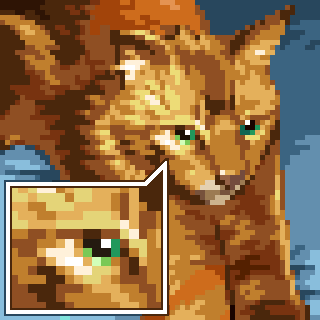
\includegraphics[width=0.9\marginparwidth]{../week2/figures/CatPixels.pdf}
  \caption{Every image you see on a computer screen is made up of tiny lights called \term{pixels}
    arranged in a grid. If you carefully look at your computer screen, you may be able to see the
    individual pixels. By turning the lights on and off and adjusting the color, the computer can
    display any image, such as this one of a cat.  \attribution{Original: ReffPixels?Vector:
      OmegaFallon, CC BY-SA 4.0 <\url{https://creativecommons.org/licenses/by-sa/4.0}>, via
      Wikimedia Commons}}
  \label{fig:pixels}
\end{marginfigure}

The purpose of providing instructions is so that we can do the same thing over again. Above, we
created a precise description of a square. Now we need to figure out a way to re-use it again and
again so we never have to write it out again!

The first way to re-use rules is to save them into a \term{file}. We call rules that we save on a
computer \term{source code}.

Let's try saving a rule. Open up Thonny and, instead of the prompt, point your mouse at the editor
(\prettyref{fig:thonny-interface}). Rules that we type here can be saved on the computer.
\hint{You can also access all these files on the internet at \url{\giturl}.\\
\begin{center}
\qrcode{\giturl}
\end{center}
}

\aside{\textcolor{red}{TODO DESCRIBE HOW TO LOAD THE FILE}}
\begin{TryThisBox}
  Type the following into the editor and then save it in a file named
  \texttt{model.py}.
  \begin{lstlisting}
draw.draw(<ENTER>
  draw.color('blue') +<ENTER>
  draw.forward(n) + draw.turn('right') +<ENTER>
  draw.forward(n) + draw.turn('right') +<ENTER>
  draw.forward(n) + draw.turn('right') +<ENTER>
  draw.forward(n)
)<ENTER>
\end{lstlisting}
\end{TryThisBox}
\hint{From now on, all the rules we see will be
    \emph{colored}. You don't need to enter the colors in. The colors
    only serve to make the rules easier to read. This is called
    \term{syntax highlighting}.}

Let's try using it:

% TODO describe how to load the file

You should get something like this:

\includegraphics[width=0.8\linewidth]{../week2/figures/onesquare.eps}\mTrackBox{Music \& Sound}{ We've seen how computers represent images as
  lights going on and off, but how do they represent \emph{sound}?

  When our ears hear sound, they are responding to \emph{changes} in
  air pressure.

  Computers represent this -- you guessed it -- using numbers!

  With graphics, we had to break up the rectangular screen into small
  chunks called pixels. For sound, we instead break up \emph{time}
  into really small sections (tens of thousands per second!) called
  samples. Within each sample, we store a number which represents the
  pressure the computer ought to output at that time. When the samples
  are sequenced together rapidly using a componenty called a DAC or
  \term{digital-to-analog converter}. }

\subsection{Introducing \kw{def} and \kw{return}}

That's good, but computers can draw squares without loading files. This is where the \kw{def}
and \kw{return} rules come in. Here's how it works.

When we have a bunch of rules we want to re-use, we can use \kw{def} to give a \emph{name} to our
rules. Then, underneath
\kw{def}, we write the rules that make up the new rule. The rules underneath have to be \term{indented}, which means that we have to type two
{\spacekey}s before typing the rule.\curious{Python is known as an \emph{indentation-aware}
language. Some languages do not care about spaces and have other ways to figure out which rules
belong as sub-rules of other rules. But for now, we'll stick with how Python does things!}

When Python follows the rules we make, it does \emph{exactly} the rules we included as part of our
named rule, but it doesn't show us the result of these rules, like what happened when we typed the
rules into the prompt directly. In order to get the final answer from our named rules, we have to
use \kw{return}.

\begin{TryThisBox}
  Type the following into \texttt{model.py}
  \begin{lstlisting}
def three_and_five():
  5
  return 3
  \end{lstlisting}
\end{TryThisBox}

Now try this in the prompt.

\begin{replbox}
three_and_five()<ENTER>
\end{replbox}

\begin{BigIdeaBox}
  We can enter as many rules as we want into \kw{def} but we have
  to use \kw{return} if we want Python to respond with a particular
  rule.
\end{BigIdeaBox}

\subsection{Combining rules}

Remember how \code{+} and \code{*} combined other rules? We can create
our own ways to combine other rules with \kw{def}. First, we have to
give names to the rules that we do not know yet. We can do this by
putting these names in parentheses after \kw{def}.\curious{These names
  for unknown rules are called \term{arguments}, even though there's
  no disagreement. Names can be funny that way!}

\begin{TryThisBox}
  \begin{lstlisting}
def mul_and_add(rule1, rule2, rule3):
  return rule1 * rule2 + rule3
  \end{lstlisting}
\end{TryThisBox}

What do you think will happen if you enter \code{mul\_and\_add(5,2,4)}
into the prompt?
%
\curious{Just like it's important to predict what will
  happen when a rule is used correctly, it's also important to think
  about what happens when rules are used incorrectly. For example,
  what do you think will happen if you entered \code{mul\_and\_add(2)}
  at the prompt?}


Let's think about it. We know what \kw{def} and \kw{return} do. When
we used \code{mul\_and\_add} at the prompt, we gave it three rules:
\code{5}, \code{2}, and \code{4}. If we look at the recipe for
\code{mul\_and\_add} above, we see that it will \kw{return} the
product of the first two rules added to the third one. So, Python's
response will be \code{14}.

We can also say that \code{mul\_and\_add(5,2,4)} \term{evaluates} to
\code{14}. Also, from now on, we will call all the ``recipes'' we make
\term{functions}.

\begin{DeepDiveBox}
  % TODO: The Stack
\end{DeepDiveBox}

\subsection{Complex Rules}

Functions allow us to combine rules. For example, we can use one
function from another. This is known as \term{calling} the function.

By using functions in this way, we can create very complex rule
systems.  \didyouknow{Just like the modeling clay we used at the
  beginning of this class could be used to model any object, we can
  use plain functions to model any system. There's an entire
  discipline of computer science that deals with this idea called
  \term{functional programming}. It's the programmer equivalent of
  playing with Play-doh, but maybe not as messy!}

\section{Drawing with Turtle}

Let's try to apply what we've learned so far by learning how to draw
with Python. As part of the course code, there is a source file named
\texttt{week2/draw.py} which contains a simple \term{library} of
functions that help us make drawings in Python. Let's try using it!

To use a Python library (also called a \term{module}) we use
\kw{import}. In the prompt type:

\begin{replbox}
import week2.draw as draw<ENTER>
\end{replbox}

We can now use functions in the module.
\curious{What do you think would happen if we
  wrote\code{import week2.draw as week2}?
  Would the other code work? How would we have to change the code to
  make it work with this new \kw{import}?}

\begin{replbox}
draw.draw(draw.forward(100))<ENTER>
\end{replbox}

You should see a line on your screen. Congratulations, you've
programmed your first picture!

The drawing system here is based off of an older programming language
called Turtle. Turtle has a few simple rules, which are listed in
\prettyref{tab:turtle}.

But to really understand Turtle, we first have to understand how we
can talk about a computer screen.

\subsection{Introduction to Computer Graphics}

%\curious{Some mathematicians think
%  there are numbers we cannot quite name. The first person to think of
%  this was a mathematician named \textbf{George Cantor}. If such a
%  number cannot be written, can you think of it? What about write a
%  description of it?}

\subsection{Drawing Our First Image}

Let's try writing a function to draw a square. Go to your Thonny
editor and try writing a function to draw a square. It would probably
look like the one below:

\begin{TryThisBox}
\end{TryThisBox}

Nice! Now, let's see if we can draw more than one square. We'll also
give our squares some color so that we can tell them apart.

\begin{replbox}
draw.draw(
  draw.color('blue') + square(200) +
  draw.color('red') + square(100))<ENTER>
\end{replbox}

\includegraphics[width=0.8\linewidth]{../week2/figures/twosquares1.eps}

We were able to combine our rules together to draw more than one
square and save us writing twice the amount of code. But hold one, the
second square appeared in a \emph{different} position than the first
one. To understand, let's ask Python to pause before it draws the
squares. Maybe we can figure out what is going on.

\begin{replbox}
draw.draw(draw.pause('square 1') + draw.color('blue') + square(200) + draw.pause('square 2') + draw.color('red') + square(200)
\end{replbox}

When you run this in the prompt, Python will \emph{pause} before each
square is drawn and wait for you to type \enterkey in the prompt
before it continues drawing.  \hint{You can always get back to the
  prompt and quit what you're currently doing by holding down both
  \controlkey and \litkey{C}. This is known as an \emph{interrupt}.}

You should get something like \prettyref{fig:twosquares-debug}.

\begin{figure}
  \fixfigure
  \label{fig:twosquares-debug}
  \centering
  \begin{minipage}{0.48\linewidth}
    \centering
    \includegraphics[width=\linewidth]{../week2/figures/twosquares-debug-square 1.eps}\\
    The First Square
  \end{minipage}
  \hfill
  \begin{minipage}{0.48\linewidth}
    \centering
    \includegraphics[width=\linewidth]{../week2/figures/twosquares-debug-square 2.eps}\\
    The Second Square
  \end{minipage}
  \caption{What it looks like before each square is drawn. Can you
    spot the difference?

    \textbf{Hint:} Look at the arrow.}
\end{figure}


What do you notice about the arrow? In Turtle, this arrow is called
the \emph{cursor} and its direction changes how \code{draw.forward}
works. If the arrow is pointing right, then \code{draw.forward} draws
to the right. Similarly, if the arrow is pointing towards the top,
then \code{draw.forward} draws towards the top. If you look at the
arrow, you'll notice that, before the first square, it points right,
and before the second, it points upward.

How do we fix this issue? The cursor starts pointing right by
default. It points upward after the first square is drawn using the
\code{square} function. How do we get it to point right again? Can you
think of an answer?

\begin{BigIdeaBox}
  Sometimes, when combining programs together, things don't work the
  way we expect because our mental model of how the computer ought to
  have done something doesn't match the exact set of rules the
  computer followed.

  It often helps to use tools like \code{draw.pause} to inspect what
  is happening in the middle of our program. This is called
  \term{debugging}.
\end{BigIdeaBox}

Here's the solution (pay attention to the italicized part!)

\begin{TryThisBox}
  \begin{lstlisting}
def square(n):
  return \
    draw.forward(n) + draw.turn('right') + \
    draw.forward(n) + draw.turn('right') + \
    draw.forward(n) + draw.turn('right') + \
    draw.forward(n)@@ + draw.turn('right')@@
  \end{lstlisting}
\end{TryThisBox}

Now, our squares are drawn the same way, but they overlap:

\includegraphics[width=0.8\textwidth]{../week2/figures/twosquares-fixed.eps}

There's only one problem now, which is that our squares all start at
the same spot. Can we move them? The answer is yes, using \code{draw.goto}.

\begin{replbox}
draw.draw(draw.color('blue') + square(200) + \<ENTER>
  draw.goto(50,50) + draw.color('red') + \<ENTER>
  square(100))<ENTER>
\end{replbox}

\subsection{A More Complicated Example}

Squares and lines are interesting, but it would be hard to do a lot of
interesting drawing using just those. Let's look at some other shapes.

The first shape we'll introduce is a \emph{circle}. A circle is defined by its radius, which is half the total distance across the circle. For example, to draw a circle with a 30 unit radius, we can use \code{draw.circle(30)}. Try this and see what happens.

\begin{replbox}
  draw.draw(draw.circle(30))
\end{replbox}

But there's more, you can also draw \emph{parts} of a circle. This is
called an \emph{arc}. To draw an arc, you can use
\code{draw.circle(30, 1/2)}, which will only draw \emph{half} the
circle\hint{You can use \code{1/2} or \code{0.5}. Python understands
  both.}

\begin{replbox}
draw.draw(draw.circle(30, 0.5))<ENTER>
draw.draw(draw.circle(40, 1))<ENTER>
draw.draw(draw.circle(20, 1/3))<ENTER>
\end{replbox}

Now, try drawing this figure.

\includegraphics[width=0.5\textwidth]{../week2/figures/lrcircle.eps}

Having trouble? Think back to the examples we tried above. Which way
did the arrow move when drawing the circle?

Turtle assumes that when we want a circle, we always want to draw it in this direction
(counter-clockwise). To make it draw in a clockwise direction, we supply it a \emph{negative} radius
(see \prettyref{fig:turtle-circles}). This arrangement where a computer system always does things
one way and requires the programmer to explicitly choose another way is called a \term{default}.

\begin{figure}[b]
  \fixfigure
  \label{fig:turtle-circles}
  \caption{The \code{draw.circle} rule produces some portion of a circle with a particular radius,
    as illustrated above. A positive radius corresponds to a point to the ``left'' of the cursors
    direction. A negative radius means to go to the right.}
  \begin{tikzpicture}[font={\sffamily\footnotesize}]
    \pgfmathsetmacro{\angleone}{2 * pi/360 * -100}
    \pgfmathsetmacro{\circleportion}{0.15}
    \pgfmathsetmacro{\circleportiontwo}{0.6}
    \pgfmathsetmacro{\circleportiontworad}{\circleportiontwo * 2 * pi}
    \pgfmathsetmacro{\circleportionrad}{\circleportion * 2 * pi}

    \pgfmathsetmacro{\circleonefinalangle}{\angleone+\circleportionrad}
    \pgfmathsetmacro{\midx}{cos(\circleonefinalangle r) * 2}
    \pgfmathsetmacro{\midy}{sin(\circleonefinalangle r) * 2}
    \pgfmathsetmacro{\circletwox}{cos(\circleonefinalangle r) * 3}
    \pgfmathsetmacro{\circletwoy}{sin(\circleonefinalangle r) * 3}
    \pgfmathsetmacro{\circletwostart}{acos(\midx - \circletwox)}
    \pgfmathsetmacro{\finalx}{\circletwox + cos((\circletwostart + \circleportiontworad) r)}
    \pgfmathsetmacro{\finaly}{\circletwoy + sin((\circletwostart + \circleportiontworad) r)}

    \draw[magenta, thick, dashed] (0,0) circle (2);
    \draw[violet, thick, dashed] (\circletwox,\circletwoy) circle(1);

    \draw[->,dashed,color=IdeaBlue] ({cos(\angleone r) * 2}, {sin(\angleone r) * 2}) -- (0, 0);
    \draw[->,dashed,color=IdeaBlue] (\finalx, \finaly) -- (\circletwox, \circletwoy);

    \draw[decorate, decoration={brace, amplitude=5pt, mirror, raise=0.2em}] (0,0) -- ({cos(\angleone r) * 1.9}, {sin(\angleone r) * 1.9}) node[midway, xshift=-2.1em] {$r = 30$};
    \draw[decorate, decoration={brace, amplitude=5pt, raise=0.3em}] ({\finalx * 0.98}, {\finaly * 0.98}) -- (\circletwox, \circletwoy) node[midway, xshift=-1.5em, yshift=-1.5em] {$r = -15$};

    \draw[black, ultra thick, {Stealth[reversed]}-{Stealth}] ({cos(\angleone r) * 2}, {sin(\angleone r) * 2}) arc ({deg(\angleone)}:{deg(\circleportionrad + \angleone)}:2) node[midway,name=arc] {};
    \draw[black, ultra thick, {Stealth-}] (\finalx,\finaly) arc
                                                    ({deg(\circletwostart+\circleportiontworad)}:{deg(2 * pi + \circletwostart) + 13}:1) node[midway,name=arctwo]{};
    \draw[dashed,xshift=0.3em,yshift=-0.3em, <-] (arc) to [bend left] ++(-2em, -4em) node[below] {\texttt{draw.circle(30, \circleportion)}};
    \draw[dashed,xshift=0.3em,yshift=0.3em, <-] (arctwo) to [bend right] ++(4em,2em) node[above] {\texttt{draw.circle(-15, \circleportiontwo)}};

\end{tikzpicture}

\end{figure}

To draw the diagram, use this code:
\curious{Try using \code{draw.pause} to visualize exactly which
  portion is drawn by which command!}
\begin{replbox}
draw.draw(draw.circle(30, 1/2) + draw.circle(-30, 1/2))
\end{replbox}

With these shapes, we can make more complicated figures. There's just
one thing left: adding color.

We saw how to change the color of the lines we drew, but how do we
\emph{fill} the shapes we draw with a color?

The \code{draw} module provides the \code{draw.fill} rule to create
filled diagrams. Let's try it.

\begin{replbox}
draw.draw(draw.fill('blue', draw.square(100)))<ENTER>
\end{replbox}

\section{The Duck Challenge}

Remember how we built that duck out of play-doh at the beginning of
the class? Everyone chose different things to focus on. Now it's time
to teach a computer to do what you did.

\begin{TryThisBox}
  Try using what you've learned thus far to draw a duck using \kw{def}
  and \kw{return} and Turtle. Name your function \code{duck}.

  As you're doing this, try to keep re-usable parts of your duck in
  separate functions, so you don't have to copy the code.
\end{TryThisBox}

Here are some examples of what you may have created. All of these are
examples of a ``duck'' that you can make using the simple rules for
drawing we learned above.

\begin{BigIdeaBox}
  To the computer, there is no duck. It's just a set of rules you told
  it to follow to draw one depiction of a duck that you found
  useful. All computer programming requires us to understand the
  problem we're trying to solve.
\end{BigIdeaBox}

\section{Copying Ducks}

You've now drawn \emph{one} duck; what if we wanted more? The whole
point of this was to codify exactly how to make a duck and explain
that to the computer. Now, with these instructions in hand, we can
make more ducks. Let's get started.

\begin{replbox}
from week2.examples import *<ENTER>
lake_of(duck)
\end{replbox}

Nice! Look at all those ducks. But, there's one problem... all our
ducks look the same. Can we make each one a bit more unique?

Let's add some \term{arguments} to our \code{duck} function. Modify
your function to include some arguments.
\begin{TryThisBox}
  \begin{lstlisting}
def duck(@@body_color@@, @@eye_color@@):
  @@your code@@
  \end{lstlisting}
\end{TryThisBox}

Now, take these arguments and use it to change your duck's body and
eye color using the \code{draw.color} and \code{draw.fill} functions
we saw above.

Now, rerun the example above:

\begin{replbox}
from week2.examples import *<ENTER>
lake_of(duck)
\end{replbox}

Much better!

\begin{BigIdeaBox}
  Since we packaged our duck into a function and added arguments to
  allow certain parts to change, we made it trivial to re-use our duck
  many times. This is a foundational part of computer programming.
\end{BigIdeaBox}

\section{Conclusion: From Drawing to Computation}

In this lesson we learned that we can often do things by hand that
take effort to describe to the computer. But once we undertake that
effort, we can use the computer to simulate things that we could not
do by hand. By expressing our duck as sets of numerical rules, we
could hand it to a computer -- a machine that follows rules -- and
manipulate it in new ways. Even though the computer couldn't
\emph{understand} the duck, it could still do useful things with our
description.

Everything in computer science is a description of something real
(whether a physical item or a real problem) that we want to solve. To
be able to manipulate this thing with computers we have to be able to
express our problem as rules the computer understands. In the case of
visual information, it means understanding graphics like the Turtle
system. In the next chapters, we'll explore other ways of describing
the world to a computer.

\Exercises

\begin{exercises}
\item Try creating some other animal as a Python function, and using
  it with the \code{lake\_of} function we used before. What does this
  show about Python's \emph{understanding} of the thing we drew?
  \answer{Whichever animal we draw, Python and the lake\_of
    function treat it the same way. Each animal is just a rule
    for Python to draw.}

\item Can you think of how the \code{lake\_of} function is able to make
  our simple image appear as if it were moving? Are there any rules
  that would create the animation sequence of each duck?

  \answer{TODO}
\end{exercises}

% Show red and blue yin/yan thing
% # ============================================================
% # Chapter 2 TODO Outline (Technical-first)
% # ============================================================
% 
% * Drawing Primitives (Missing Technical Core) - Done
% - Introduce arcs / circles as drawing primitives - Done
% - Show how arcs differ from straight lines - Done
% - Explain radius + angle intuitively (no formulas yet) - Need to ADD diagram
% - Add example: combining lines + arcs -- NOT DONE
% - Add figure showing arc parameters visually -- TODO
% 
% * Filling and Regions -- DONE
% - Introduce closed shapes -- TODO
% - Explain what ?inside? vs ?outside? means -- TODO
% - Introduce fill as coloring a region - DONE
% - Show same outline with and without fill - Add diagram TODO
% 
% * Multiple Duck Representations (Technical)
%     - Draw duck using only lines
%     - Draw duck using lines + arcs
%     - Draw duck using fill
% - Compare versions side-by-side
% - Ask: what details were added / removed?
% 
% * Modeling Choices -- will not do
% - Explicitly name ?model? at this point
% - Identify what each duck drawing ignores -- figure caption
% - Identify what each drawing keeps -- figure caption
% - Add diagram: same duck, different models
% 
% * Simulation: A Lake of Ducks
% - Introduce idea of many ducks, same rules -- done
% - Add simple rule-based placement (position, size, direction)
% - Show variation via parameters -- done
% - Simulate multiple ducks on a lake
% - Add figure: single duck vs many ducks
% 
% * Abstraction via Parameters -- colors of body, and eyes
% - Name parameters explicitly -- 
% - Show how changing numbers canges appearance -- TODO
% - Connect parameters to ?knobvs? on the model -- no
% 
% * From Drawing to Computation
% - State: computer draws by following rules
% - Emphasize repeatability
% - Emphasize no understanding of ?duck?
% 
% * Curiosity / Track Boxes (Insert Where Natural)
% - Graphics: circles aren?t really circles
% - Games: fake physics
% - Sound: sound as numbers
% - Simulation: same rules, many agents
% 
% * Conceptual Wrap-Up
% - Revisit duck question one last time
% - State: model ? thing
% - State: computers work only with models
% - End with forward-looking question
% 
% # ============================================================
